
% ********** Chapter 5 **********
\chapter{Application Overview}
\label{sec:WebCallSDKArchitecture}

\section{Use Cases}

\textbf{TODO: write some use cases as well as figures here}


\section{Architecture Overview}
\label{sec:WebCallSDKArchitecture:ArchitectureOverview}

This chapter presents a brief solution description of Web Call SDK. The design architecture is shown in Figure \ref{fig:ArchitectureOfWebCallSDK}.

\begin{figure}[!hbtp]
\centering
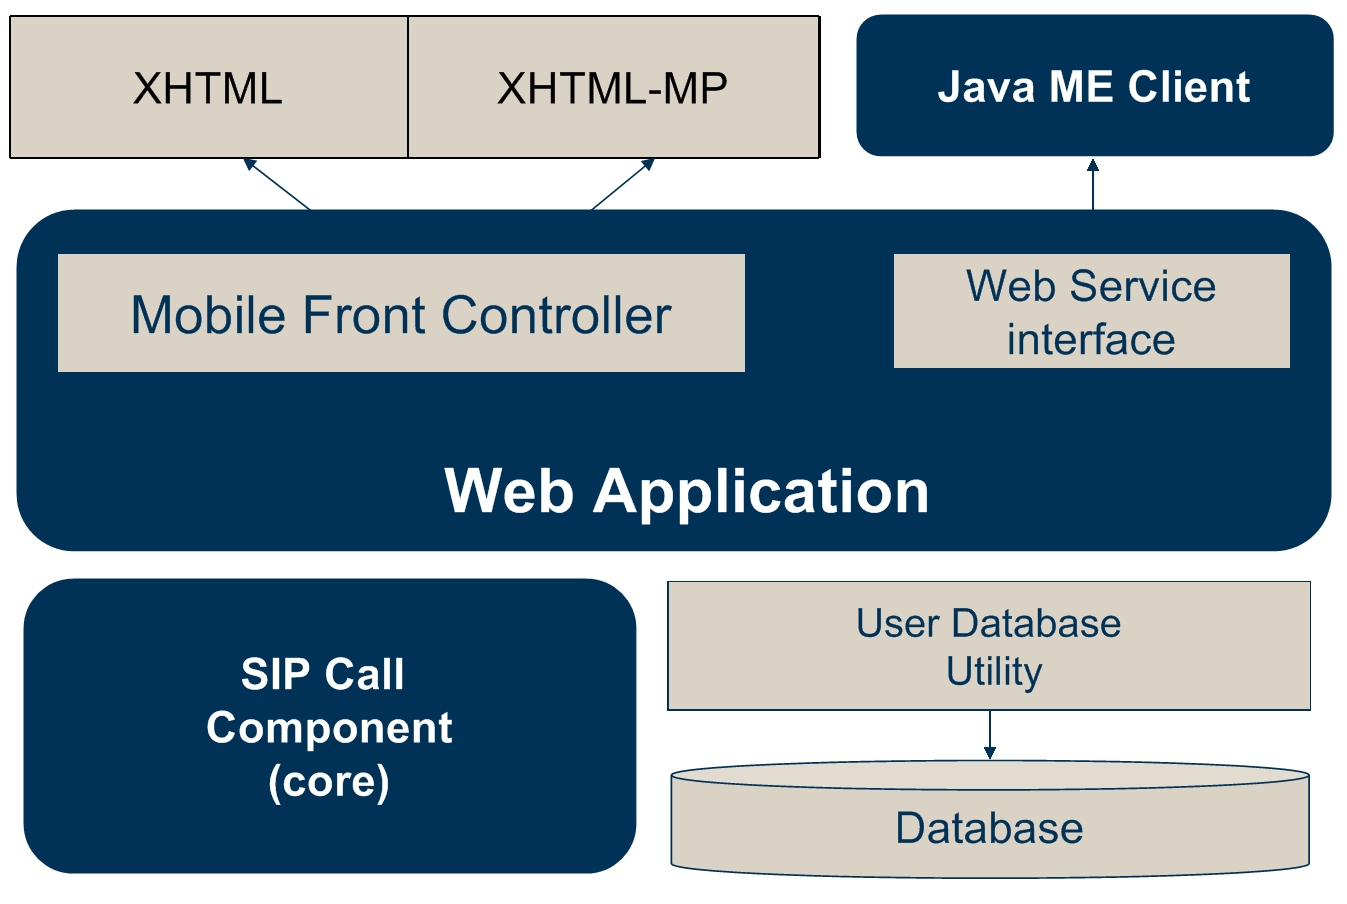
\epsfig{file=chap05/resources/architecture, width=5.2in}
\caption{The Architecture of Web Call SDK}
\label{fig:ArchitectureOfWebCallSDK}
\end{figure}

Web Call SDK contains three components which are SIP Call Component, Web Application (include web service interface) and Java ME client. The three components are shown with dark blue back ground in Figure \ref{fig:ArchitectureOfWebCallSDK}.

\subsection{SIP Call Component}

The SIP Call Component is the core of Web Call SDK. It implemented 1 kind of relay call and four kind of third party call. It can be also used as a stand alone VoIP high-level API. 

The details about SIP Call Component will be described in Chapter \ref{sec:SIPCallComponent}.

\subsection{Web Application}

The Web Application is built on the architecture of Mobile Front Controller (MFC). SIP Call Component integrated into the web server as Java EE components: servlet, and web service. The Mobile Front Controller is used for detecting and selecting views, i.e. applications with views for desktop and mobile browsers. So Web Call Example Application supplies both XHTML view which used by desktop browser and XHTML-MP view which used by mobile browser. 

The details about Web Application will be described in Chapter \ref{sec:WebApplication}.

\subsection{Web Service Interface}

The web service interface in web application supplies a common interface for using sip call function. It uses a same database as MFC based Web Application.

The details about Web Service Interface will be described in Chapter \ref{sec:WebServiceInterface}.

\subsection{Java ME client}

Java ME client is a client of web service interface. It not only implement all of the client side function of web service interface, but also include some convenient function such as read phone contact book and synchronize with server contact book.

The details about Java ME client will be described in Chapter \ref{sec:JavaMEClient}.







% ********** End of chapter **********
